\section{Parallelization}
\begin{frame}{\st{Serial} Parallel Version}
    The Huffman Compression Algorithm is composed by four phases:
    \begin{enumerate}
        \item \textbf{Count} the byte frequencies
        \item Build the Huffman tree using the frequencies
        \item Generate the Huffman alphabet by visiting the Huffman tree by using a DFS algorithm
        \item \textbf{Data encoding} using the Huffman alphabet
    \end{enumerate}
    Step 1 and 4 are the most expensive and easiest to parallelize
\end{frame}
\begin{frame}{Parallelization}
    \begin{itemize}
        \item Multiple \textbf{processes} should handle separate files.
        \item Multiple \textbf{threads} of the same process should work on different chunks of the same file in parallel.
    \end{itemize}
\end{frame}
\begin{frame}{Reasoning}
    \begin{itemize}
        \item In most operating systems a file is a resource that the OS gives to a single process to avoid I/O race conditions.
        \item Because threads of the same process share the address space, we can avoid the expensive data transfer across processes.
    \end{itemize}
\end{frame}

\begin{frame}{Multithreading}
    Given $m$ threads:

    \begin{enumerate}
        \item A file is divided into $c$ \emph{chunks}, usually $m < c$ 
        \item Until all chunks are not processed:
        \begin{enumerate}
            \item A single thread reads $m$ chunks and stores them in a shared memory space
            \item Each thread works on its own assigned chunk
            \item A single thread writes the processed chunks on the disk
        \end{enumerate}
    \end{enumerate}
\end{frame}

\begin{frame}{Architecture}
    \begin{figure}
        \centering
        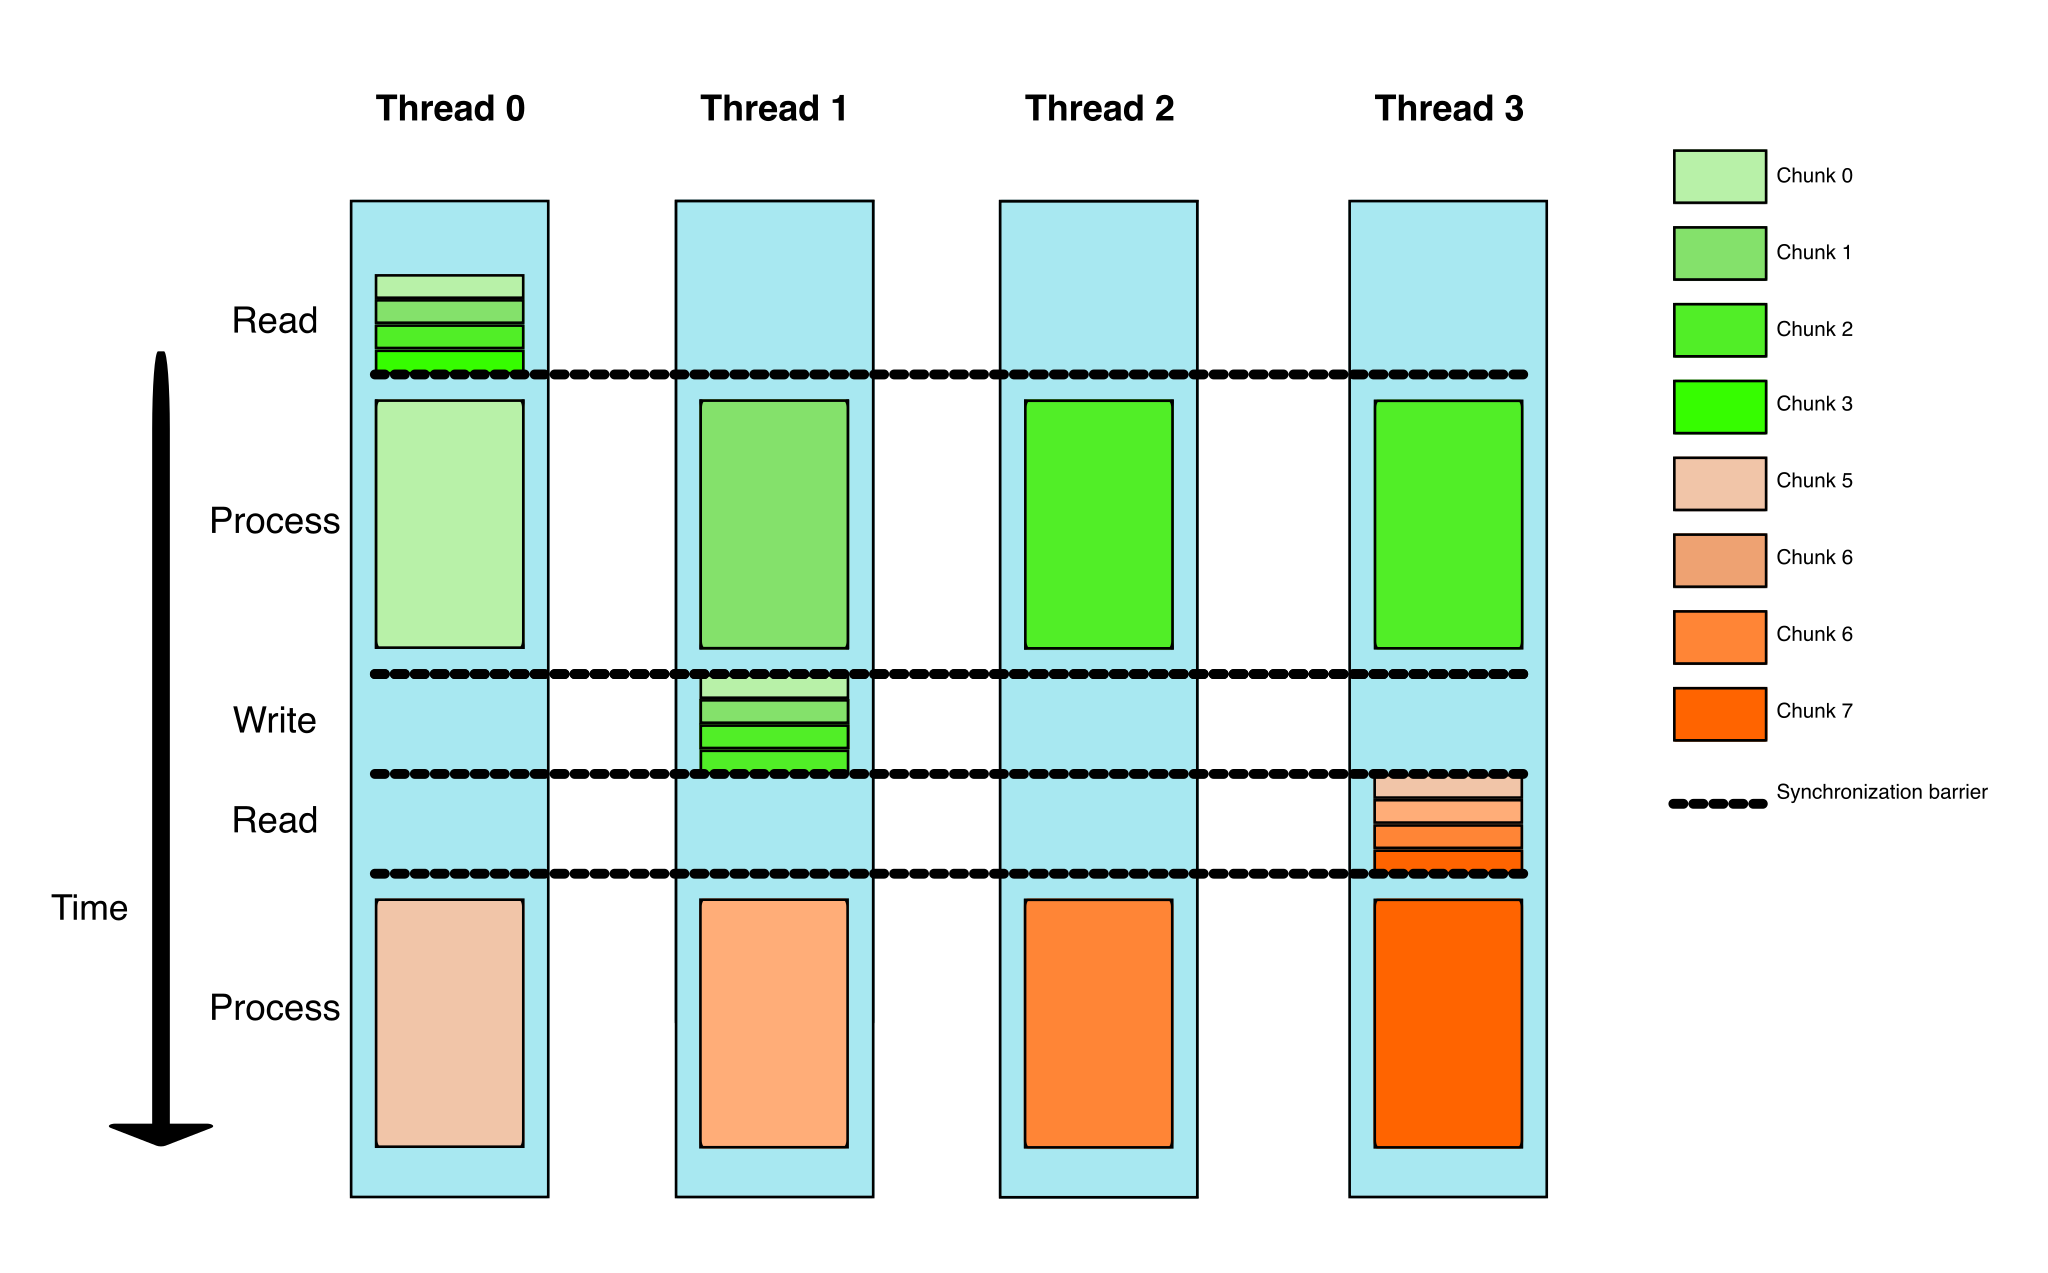
\includegraphics[width=\linewidth]{../imgs/threading}
        \caption{Simple schema for processing a single file with multiple threads.}
        \label{fig:threading}
    \end{figure}
\end{frame}
  \begin{frame}{Multiprocessing}
    \begin{itemize}
        \item Rank 0 gathers all files in the input folder
        \item Reads their size
        \item Distributes to other processes files, balancing the load using a min priority Q
        \item Each process work on its own queue of jobs 
    \end{itemize}
\end{frame}
    \begin{frame}{Multiprocess Architecture}
    \begin{figure}
        \centering
        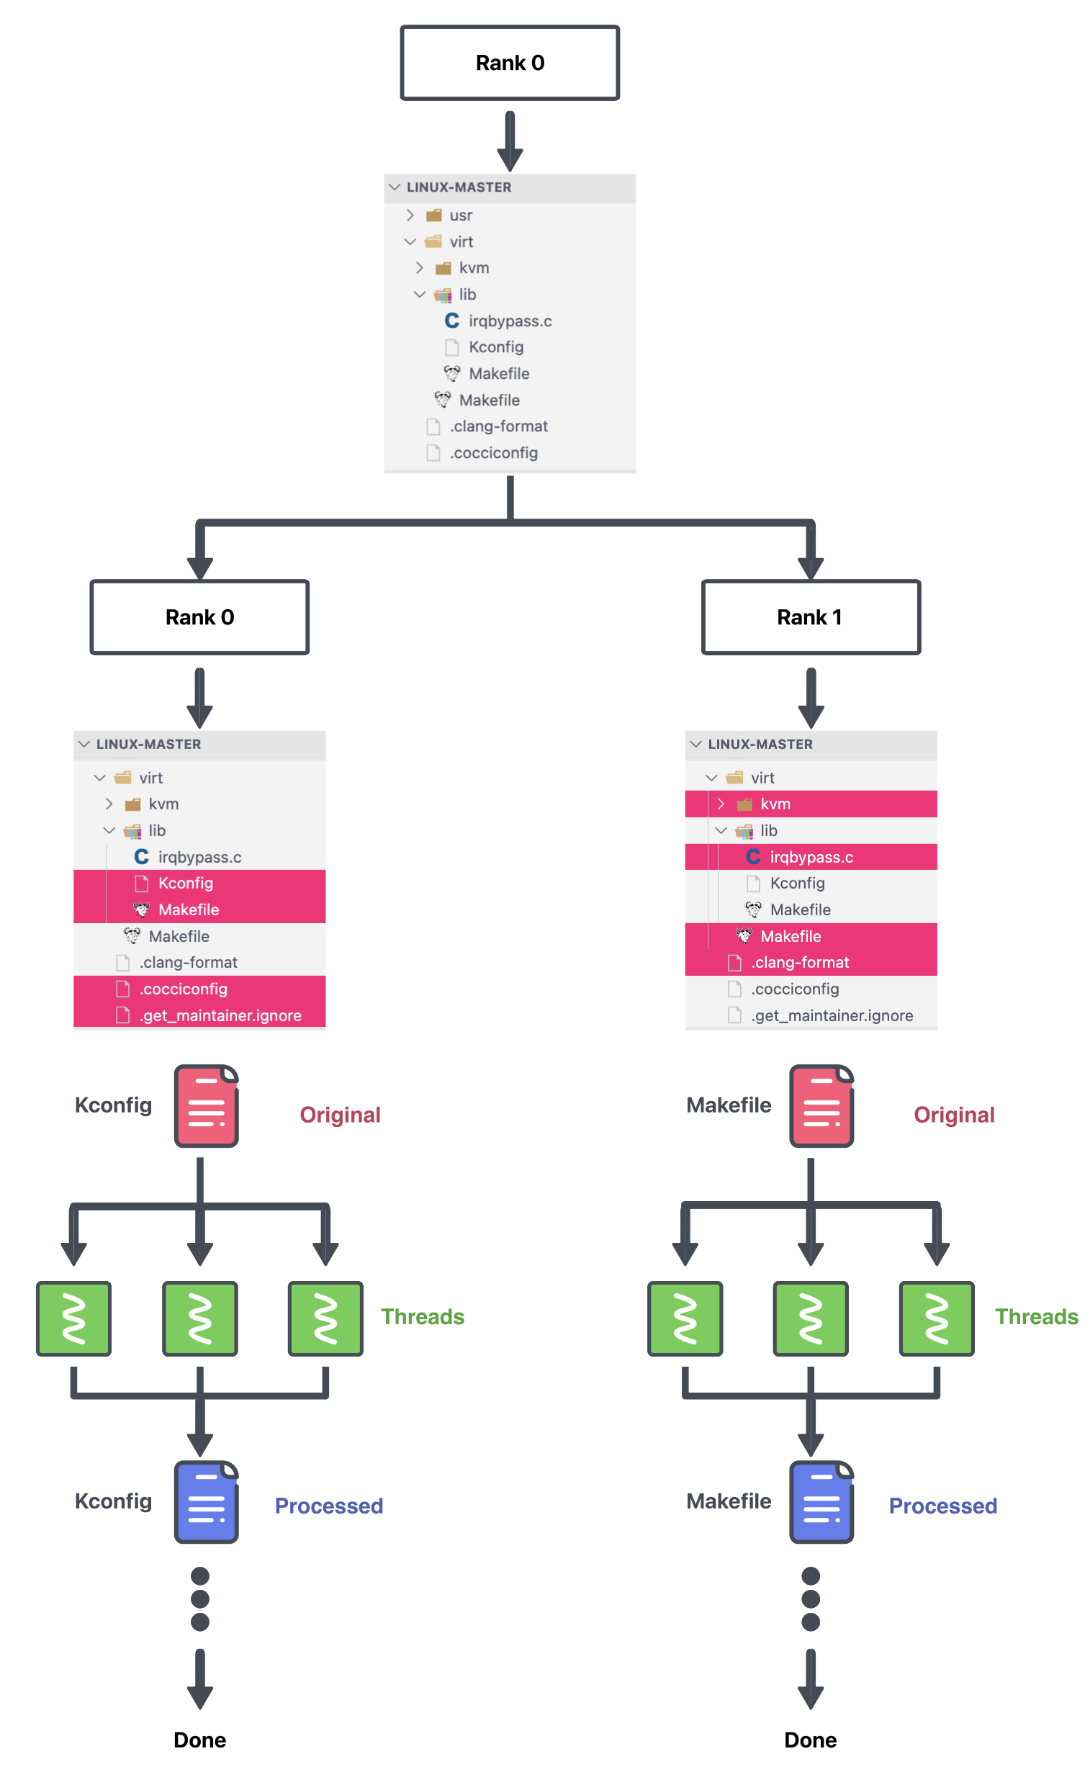
\includegraphics[width=0.40\textwidth]{../imgs/overall flow schema.png}
        \caption{Simple overall schema}
        \label{fig:threading}
    \end{figure}
\end{frame}
\begin{frame}{Implementation notes}
    \begin{itemize}
        \item 1 byte as alphabet. More bytes results in less collisions and therefore less efficiency
        \item 4096 B as chunk size, because it is the standard linux page size
        %\item I/O is not real I/O, but is a request to the OS to do the I/O
    \end{itemize}
\end{frame} 

\begin{frame}{Alternative Architecture (with Locks)}
    \begin{figure}
        \centering
        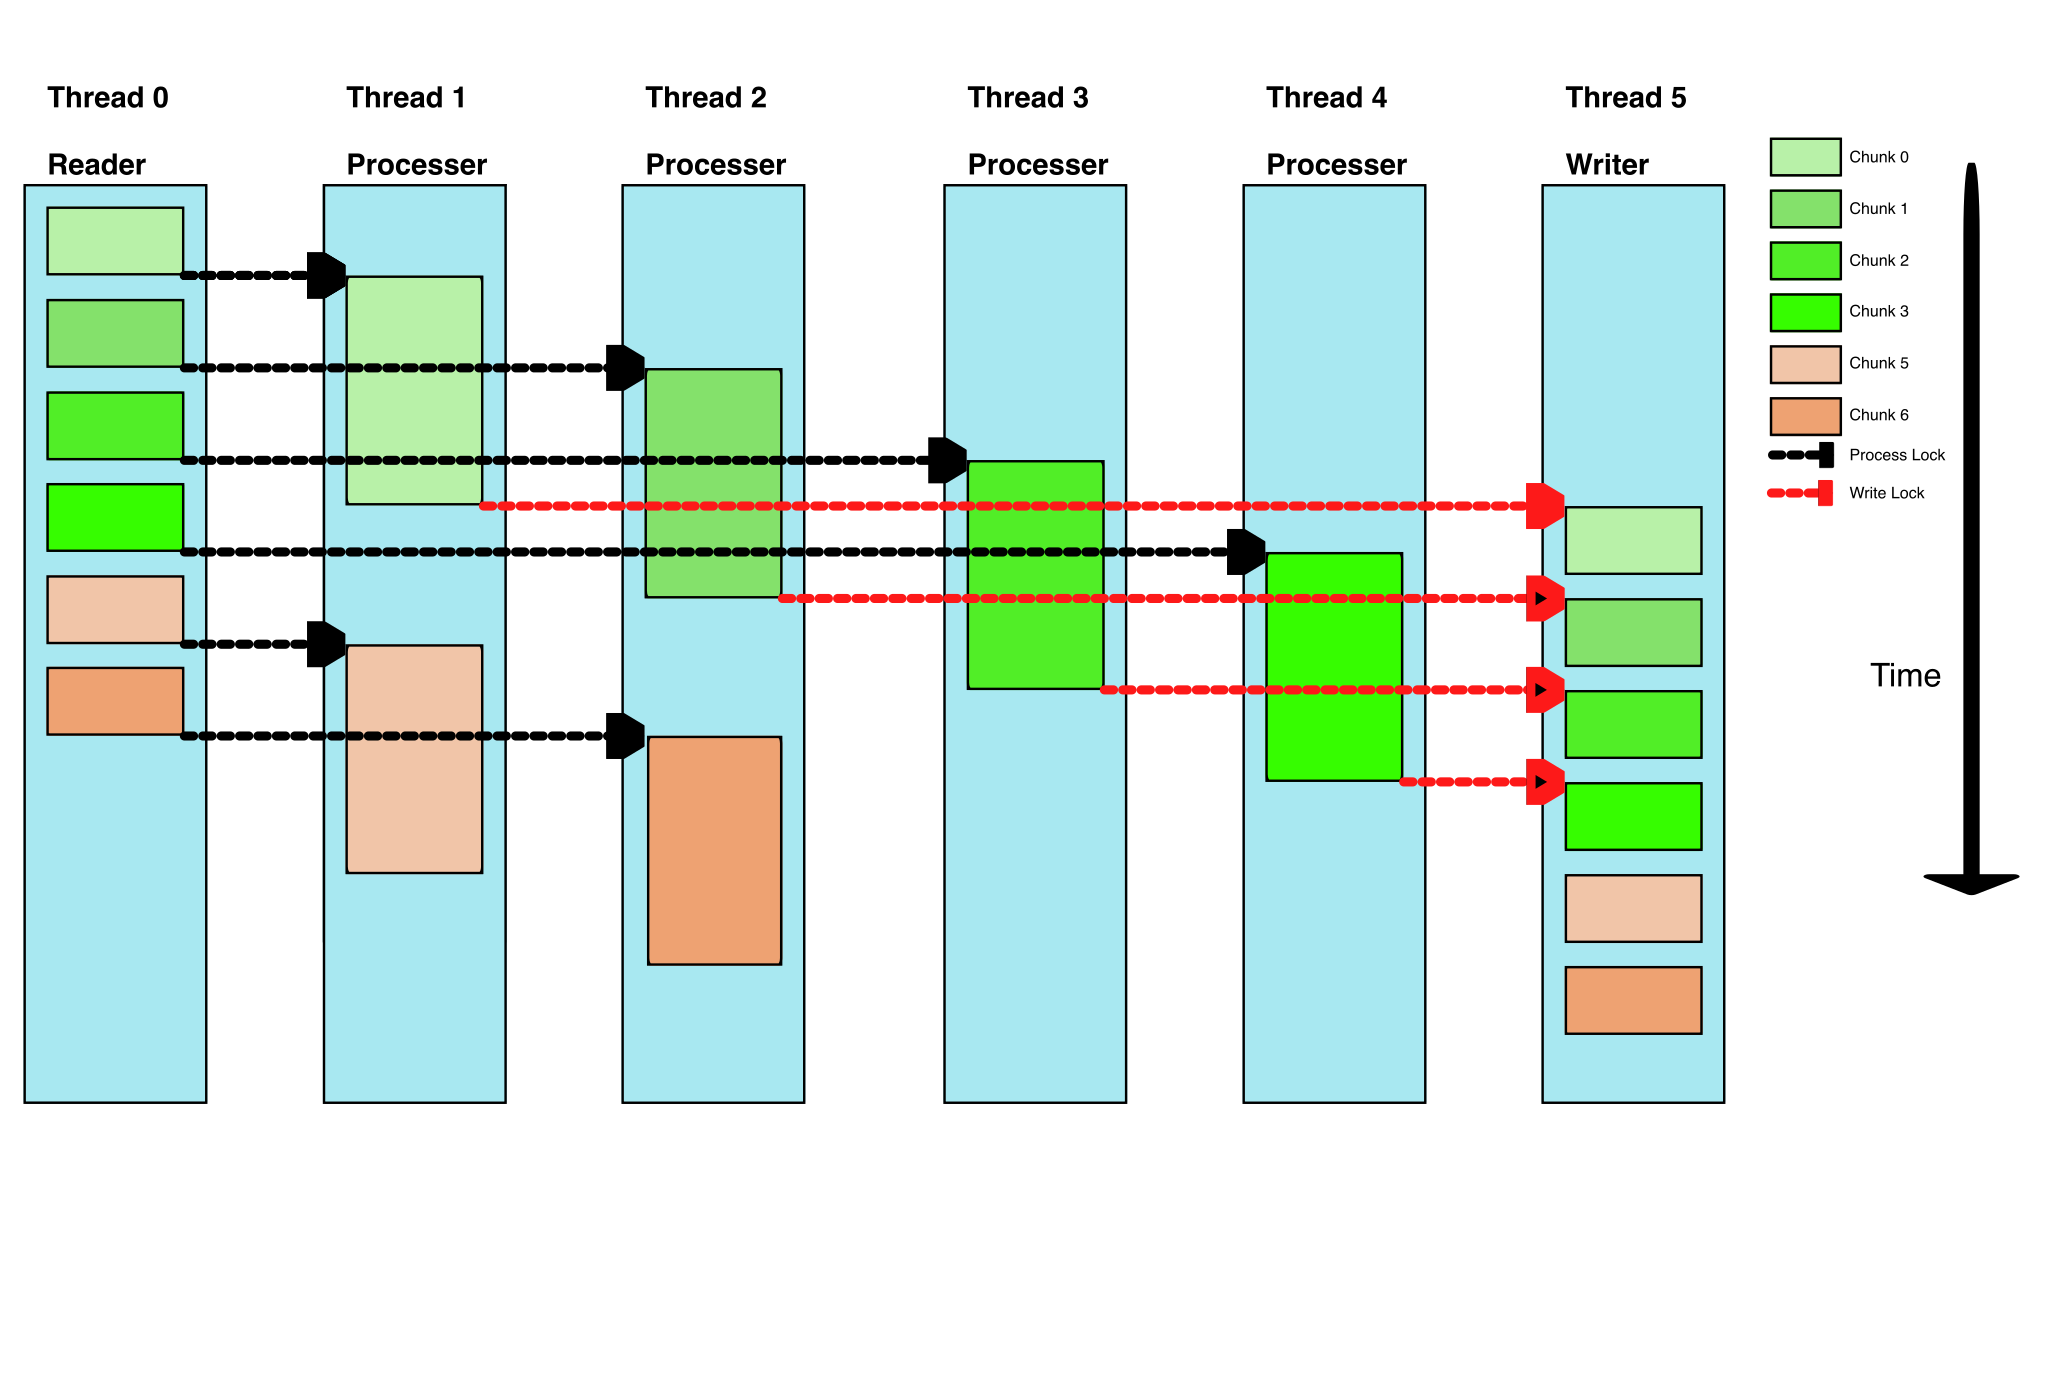
\includegraphics[width=\linewidth]{../imgs/dedicated IO threads}
        \caption{Simple schema for processing a multiple files.}
        \label{fig:threading}
    \end{figure}
\end{frame}
